\section{Classification}
\label{sec:multivariate_classification}

The $k$-class classification task involves assigning an observation $\vx$ to
one of $k$ populations, described by distributions $F_i$ for $1 \leq i \leq
k$.
The populations may also be associated with prior probabilities $\pi_i$.

\begin{definition}[Classifier]
    A classifier is a map $\hat{\iota}\colon \R^d \to \{1, \dots, k\}$.
\end{definition}

\begin{example}[Bayes classifier]
    Suppose that the population densities $f_i$ for each $1 \leq i \leq k$ are
    known.
    The Bayes classifier assigns $\vx$ to the $\hat{\iota}_B$-th population
    where
    \begin{equation}
        \hat{\iota}_B(\vx) \,=\, \argmax_{1 \leq i \leq k}\; \pi_i f_i(\vx).
    \end{equation}
\end{example}

One way of measuring the performance of a classifier (given the population
distributions and their priors) is by measuring its average misclassification
rate.

\begin{definition}[Average misclassification rate]
    The average misclassification rate of a classifier $\hat{\iota}$ is given
    by
    \begin{equation}
        \Delta(\hat{\iota}) \,=\, \sum_{i = 1}^k\, \pi_i\,P_{\vX \sim F_i}(\hat{\iota}(\vX) \neq i).
    \end{equation}
\end{definition}

\begin{proposition}
    The Bayes classifier has the lowest possible average misclassification
    rate. This is known as the optimal Bayes risk, denoted $\Delta_B$.
\end{proposition}

The simplest depth based classifier is the maximum depth classifier
\parencite{ghosh-chaudhuri-2005}.

\begin{example}[Maximum depth classifier]
    Suppose that the prior probabilities $\pi_i$ are equal.
    The maximum depth classifier $\hat{\iota}_D$ for a choice of depth
    function $D$ is described by
    \begin{equation}
        \hat{\iota}_D(\vx) \,=\, \argmax_{1 \leq i \leq k}\; D(\vx, F_i).
    \end{equation}
\end{example}

In practice, instead of having direct access to the population distributions
$F_i$, we have typically deal with labeled training data
\begin{equation}
    \mathscr{D} \,=\, \{(\vx_{ij}, i)\} \subset \R^d \times \{1, \dots, k\},
\end{equation}
where $\vx_{i1}, \dots, \vx_{in_i}$ is an instance of an iid sample from $F_i$
for each $1 \leq i \leq k$.
The empirical maximum depth classifier simply replaces the population
distributions $F_i$ with their empirical counterparts $\hat{F}_i$ determined
by $\vx_{i1}, \dots, \vx_{in_i}$. Thus, it is given by
\begin{equation}
    \hat{\iota}_{D}(\vx) \,=\, \argmax_{1 \leq i \leq k}\; D(\vx, \hat{F}_i).
\end{equation}
Under certain restrictions, this classifier becomes asymptotically optimal in
the following sense.

\begin{theorem}[\cite{ghosh-chaudhuri-2005}]
    Suppose that the population density functions $f_i$ are elliptically
    symmetric, with $f_i(\vx) = g(\vx - \vmu_i)$ for parameters $\vmu_i$ and a
    density function $g$ such that $g(k\vx) \leq g(\vx)$ for every $\vx$ and
    $k > 1$. Further suppose that the priors on the populations are equal, and
    the depth function $D$ is one of HD, SD, MJD, PD. Then,
    $\Delta(\hat{\iota}_{D}) \to \Delta_B$ as $\min\{n_1, \dots,
    n_k\} \to \infty$.
\end{theorem}

Note that this result deals with elliptic population densities differing only
in location.
Relax this assumption, and instead suppose that $f_i \sim \Ell(h_i; \vmu_i,
\Sigma)$, i.e.
\begin{equation}
    f_i(\vx) = c_i |\Sigma|^{-1/2} h_i\left((\vx - \vmu_i)^\top \Sigma^{-1} (\vx - \vmu_i)\right)
\end{equation}
for strictly decreasing $h_i$, and that the depths can be expressed as
$D(\Cdot, F_i) = l_i(f_i(\Cdot))$ for strictly increasing functions $l_i$.
It follows that the Bayes decision rule can be reformulated as
\begin{equation}
    \pi_i f_i(\vx) > \pi_j f_j(\vx) \;\iff\; D(\vx, F_i) > r_{ij}(D(\vx, F_j))
\end{equation}
for some real increasing function $r_{ij}$.
Using this observation, the DD classifier \parencite{li-albertos-liu-2012}
picks separating functions $r_{ij}$ which best classify the training data
$\mathscr{D}$.

\begin{definition}[Empirical misclassification rate]
    The empirical misclassification rate of a classifier $\hat{\iota}$, with
    respect to data $\mathscr{D}$, is given by
    \begin{equation}
        \hat{\Delta}(\hat{\iota}) \,=\, \sum_{i = 1}^k \frac{\pi_i}{n_i}\sum_{j = 1}^{n_i} \bm{1}(\hat{\iota}(\vx_{ij}) \neq i).
    \end{equation}
\end{definition}


\begin{figure}
    \centering
    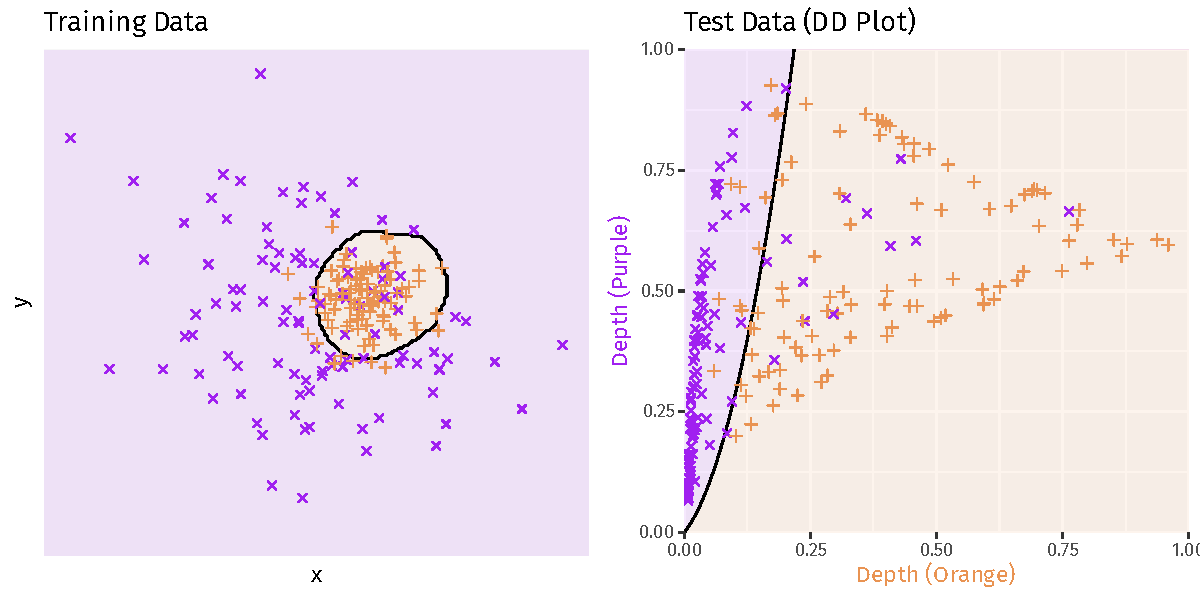
\includegraphics[width = \textwidth, page = 1]{classify}
    \caption{
        The DD classifier using spatial depth and a polynomial separating
        curve.
        The orange and purple shaded regions indicate the prediction rule
        learned from the training data; the black line marks the separating
        boundary.
        The classification accuracy here is 88\%.
    }
    \label{fig:dd_classifier}
\end{figure}


\begin{definition}[DD classifier]
    Suppose that $k = 2$, that $D$ is a depth function, and that $r\colon [0,
    1] \to [0, 1]$ is an increasing function. The DD classifier
    $\hat{\iota}_{D, r}$ is given by
    \begin{equation}
        \hat{\iota}_{D, r}(\vx) \,=\, \begin{cases}
            1, &\text{ if } D(\vx, F_2) \leq r(D(\vx, F_1)), \\
            2, &\text{ if } D(\vx, F_2) >    r(D(\vx, F_1)).
        \end{cases}
    \end{equation}
    % The optimal separating curve $r$ is chosen from a family of curves
    % $\Gamma$ so as to minimize the average classification error, i.e.\ \[
    %     r = \argmin_{r' \in \Gamma} \Delta(\hat{\iota}_{D, r'}).
    % \]
    The empirical DD classifier $\hat{\iota}_{D, \hat{r}}$ replaces $F_i$ by
    their empirical counterparts $\hat{F}_i$.
    Here, the separating curve $\hat{r}$ is chosen from a family $\Gamma$ so
    as to minimize the empirical misclassification rate, i.e.
    \begin{equation}
        \hat{r} = \argmin_{r \in \Gamma} \hat{\Delta}(\hat{\iota}_{D, r}).
    \end{equation}
\end{definition}

Figure~\ref{fig:dd_classifier} shows the DD classifier applied on normal
populations.

\begin{remark}
    The maximum depth classifier $\hat{\iota}_D$ is simply the DD classifier
    $\hat{\iota}_{D, \id}$, where $\id(x) = x$.
    Figure~\ref{fig:ddplots_location_scale} clearly illustrates how this
    choice of separating function may not always be appropriate, especially
    when the different populations have scale differences.
\end{remark}

\textcite{li-albertos-liu-2012} show that under certain restrictions, the
empirical DD classifier is asymptotically equivalent to the Bayes rule. We
give one such instance below.

\begin{lemma}
    Suppose that the following conditions hold.
    \vspace{-1em}
    \begin{enumerate}[itemsep = -0.2em]
        \item $\Gamma$ is the class of polynomial functions on $[0, 1]$.
        \item The depth functions $D(\Cdot, F_i)$ are continuous.
        \item As $\min\{n_1, n_2\} \to \infty$, we have for each $i \in \{1, 2\}$,
        \begin{equation}
            \sup_{\vz \in \R^d} |D(\vz, \hat{F}_i) - D(\vz, F_i)| \toas 0.
        \end{equation}
        \item The distributions $F_i$ are elliptical and satisfy for all
        $\delta \in \R$
        \begin{equation}
            P_{\vZ \sim F_i}(D(\vZ, F_i) = \delta) = 0.
        \end{equation}
    \end{enumerate}
    Then, $\Delta(\hat{\iota}_{D, \hat{r}}) \to \Delta_B$ as $\min\{n_1, n_2\}
    \to \infty$.
\end{lemma}

In all the depth based classifiers we have seen so far, the classification
rule depends on the observation $\vx$ only through the depths $D(\vx, F_i)$.
Thus, we are motivated to define the following transformation from $\R^d$ to a
depth feature space.

\begin{definition}
    The depth feature vector $\vx^D$ of an observation $\vx$, with respect to
    the population distributions $F_i$ and a choice of depth function $D$, is
    defined as
    \begin{equation}
        \vx^D \,=\, \left(D(\vx, F_1), \dots, D(\vx, F_k)\right).
    \end{equation}
\end{definition}
\begin{remark}
    The graph
    \begin{equation}
        \DD(F_1, \dots, F_k) = \{\vx^D : \vx \in \R^d\}
    \end{equation}
    is the analogue of the \nameref{def:ddplot}, with $k$ distributions.
\end{remark}

Assuming that the depth function $D$ only takes values in $[0, 1]$, the map
$\vx \mapsto \vx^D$ takes values in $[0, 1]^k$, regardless of the
dimensionality of the original vector $\vx$.
With this, the maximum depth classification rule can be expressed as
\begin{equation}
    \hat{\iota}_D(\vx) = i \;\iff\; \vx^D \in R_i^D = \{\vy \in [0, 1]^k : y_i = \max_j y_j\}.
\end{equation}
Indeed, any partition of the unit cube $[0, 1]^k$ into $k$ decision regions
$R^D_i$ gives rise to a depth based classifier.
The DD classifier achieves this by using an increasing separating function
$r$ to partition $[0, 1]^2$.
Furthermore, $r \in \Gamma$ is chosen so as to best separate the training data
$\mathscr{D}$ transformed into the depth feature space.
However, we can in principle use the transformed training data
\begin{equation}
    \mathscr{D}^D \,=\, \{(\vx^D_{ij}, i)\} \subset [0, 1]^k \times \{1, \dots, k\}
\end{equation}
along with any multivariate classification algorithm (LDA, QDA, $k$NN, GLM,
etc) to devise suitable decision regions.
This is precisely the formulation of the DD$^G$ classifier
\parencite{albertos-bande-fuente-2017}.


